\documentclass{article}
\usepackage{spconf,amsmath,graphicx,booktabs,url,microtype,array,multirow}
\usepackage[T1]{fontenc}
\setlength{\emergencystretch}{2em}

\title{DATA-EFFICIENT NUCLEUS SEGMENTATION ACROSS MICROSCOPY MODALITIES}
\name{Varun Kumar Dasoju$^{1}$, Qingsu Cheng$^{2}$, Zeyun Yu$^{1}$}
\address{University of Wisconsin--Milwaukee, Milwaukee, WI, USA\\
$^{1}$Department of Computer Science; $^{2}$Department of Biomedical Engineering\\
\texttt{vdasoju@uwm.edu, chengq@uwm.edu, yuz@uwm.edu}}

\begin{document}
\maketitle

\begin{abstract}
Hand-crafted edge channels are often presented as data-efficient priors for nucleus segmentation, but their benefit over matched deep baselines and across acquisition modalities is rarely isolated. We audit an EfficientNet-B7/UNet++ pipeline and perform 114 controlled public-data training runs. On the official BBBC039 fluorescence split, a Gabor-projection-SCSE bundle obtains 96.85\% Dice versus 96.60\% for vanilla B7, a gain of 0.250 percentage points (95\% CI 0.197--0.299), but is statistically indistinguishable from UNet++/Xception/SCSE (96.87\%). On 50 TNBC H\&E images, five-fold patient-grouped cross-validation reverses the conclusion: vanilla B7 obtains 74.29\% patient-macro Dice, Xception/SCSE 73.03\%, and the Gabor bundle 67.02\%. Gabor therefore loses 7.26 points against vanilla (95\% CI $-9.98$ to $-5.26$; Holm-adjusted $p=.0039$). A fluorescence-to-histology zero-shot stress test also rises from 8.07\% to 51.30\% Dice after fixed intensity inversion, demonstrating a major polarity mismatch. A corrected audit of private UWM data finds no full-pipeline superiority. The evidence supports an acquisition-dependent, not universal, edge prior and establishes a reproducible framework for testing such priors without slice leakage, unequal budgets, or selective reporting.
\end{abstract}

\begin{keywords}
nucleus segmentation, fluorescence microscopy, breast histology, Gabor filters, reproducibility
\end{keywords}

\section{Introduction}
Nuclear masks support cell counting, morphology, spatial analysis, and downstream computational pathology. Their manual annotation is expensive, making data-efficient segmentation attractive. U-Net~\cite{ronneberger2015unet}, UNet++~\cite{zhou2018unetpp}, pretrained encoders, and generalist cell models~\cite{pachitariu2025cellposesam,archit2025microsam} nevertheless create strong controls. A proposed hand-crafted prior must therefore be compared with equally trained alternatives and evaluated outside the acquisition pattern that motivated it.

This distinction matters for the present project. It began with grayscale confocal images of mammary epithelial nuclei and combined multi-scale Gabor responses with EfficientNet-B7/UNet++, a learned input projection, and spatial/channel squeeze-and-excitation (SCSE). Fluorescence nuclei are usually bright compact objects on dark backgrounds. In H\&E breast histology, nuclei are dark, chromatically stained objects embedded in textured tissue. A filter that helps the former may amplify irrelevant stromal, cytoplasmic, or stain boundaries in the latter.

An earlier version reported 95.1\% Dice from a small private set. Peer review identified unresolved empty-image scoring, slice leakage, unequal baseline budgets, incorrect loss interpretation, missing boundary terms and metrics, insufficient Gabor sensitivity, underspecified sampling, absent confidence intervals, weak annotation documentation, and no external evaluation. The present study treats those concerns as design requirements rather than cosmetic revisions.

Our contributions are:
\begin{enumerate}
\item a reproducible evaluation with explicit native-grid metrics, empty-mask rules, matched schedules, multi-seed uncertainty, paired tests, and complete negative results;
\item 69 controlled runs on the official BBBC039 fluorescence split, including architecture, component, edge, loss, sampling, and filter-bank ablations;
\item 45 newly trained runs on TNBC using five fixed patient-disjoint outer folds, showing that the fluorescence benefit reverses on breast H\&E;
\item real input, filter-response, annotation, and held-out prediction panels for both public datasets; and
\item a transparent reconciliation of the private UWM result and a modality-shift stress test that isolates intensity polarity.
\end{enumerate}
The task is two-dimensional semantic nuclear foreground segmentation. It is not breast-cancer diagnosis, clinical validation, or instance separation.

\section{Related work}
\subsection{Fluorescence nuclei}
BBBC039 was released through the Broad Bioimage Benchmark Collection~\cite{ljosa2012annotated} and used in the 2018 Data Science Bowl analysis~\cite{caicedo2019nucleus}. Caicedo et al. compared deep-learning strategies under the official split and emphasized cross-experiment variation~\cite{caicedo2019evaluation}. Later methods include graph-based refinement in SegmentGraph~\cite{yi2022segmentgraph}, integrative shape-aware segmentation~\cite{wang2022aswnet}, and multi-dataset frameworks such as NUSeg~\cite{wickramasinghe2024nuseg}. Their published endpoints are useful context, but object F1, pixel Dice, aggregated Jaccard index (AJI), and cross-validation estimates are not interchangeable.

\subsection{Histopathology nuclei}
The TNBC set contains breast H\&E image patches and expert nuclear annotations from 11 patients~\cite{naylor2019segmentation}. Published approaches include distance-map regression~\cite{naylor2019segmentation}, stacked attention U-Nets~\cite{kang2020twostage}, multi-organ region segmentation~\cite{mahmood2021accurate}, FRE-Net~\cite{huang2023frenet}, MA-Net~\cite{alotaibi2024manet}, and few-shot adaptation~\cite{he2023celltranspose}. Reported scores use different splits, preprocessing, instance handling, and averaging units. We therefore use published values only as protocol-labelled context and make causal comparisons only among models retrained here under an identical patient-grouped protocol.

\subsection{Study gap}
Most reports ask whether a method performs well on one benchmark. Our narrower question is whether an explicit edge prior adds value after controlling architecture and whether its effect survives a change from fluorescence to breast histology. This is important because a positive single-benchmark ablation can otherwise be misread as evidence of general-purpose robustness.

\section{Method}
\subsection{Preprocessing and edge representation}
Let $x$ denote percentile-rescaled grayscale intensity. For a Gabor kernel with orientation $\theta$ and frequency $f$, the real response is
\begin{equation}
k_{\theta,f}(u,v)=\exp\left[-\frac{u'^2+\gamma^2v'^2}{2\sigma^2}\right]\cos(2\pi f u'),
\end{equation}
where $u'=u\cos\theta+v\sin\theta$, $v'=-u\sin\theta+v\cos\theta$, $\gamma=0.5$, $\sigma=5$, zero phase, and kernel size 31. The edge channel is
\begin{equation}
e(x)=\mathcal N\!\left(\max_{\theta,f}\left|x*\frac{k_{\theta,f}}{\lVert k_{\theta,f}\rVert_1+\epsilon}\right|\right),
\label{eq:gabor}
\end{equation}
using eight evenly spaced orientations, $f\in\{0.05,0.15,0.25\}$ cycles/pixel, and normalization $\mathcal N$ to $[0,1]$. L1 kernel normalization avoids the instability of normalization by a near-zero signed sum.

\subsection{Segmentation architecture}
The proposed bundle concatenates three replicated intensity channels and $e(x)$. A learned $4\!\rightarrow\!16\!\rightarrow\!8\!\rightarrow\!3$ projection preserves compatibility with an ImageNet-pretrained EfficientNet-B7 encoder~\cite{tan2019efficientnet}. A UNet++ decoder and SCSE attention~\cite{roy2018scse} produce the semantic foreground probability. Figure~\ref{fig:method} depicts the implemented path. Controls remove the edge and SCSE, retain SCSE only, replace Gabor with Sobel, or use identity-preserving residual fusion,
\begin{equation}
x_{out}=x_{RGB}+\tanh(a)P([x_{RGB},e]), \qquad a_0=0.
\end{equation}

\begin{figure*}[t]
\centering
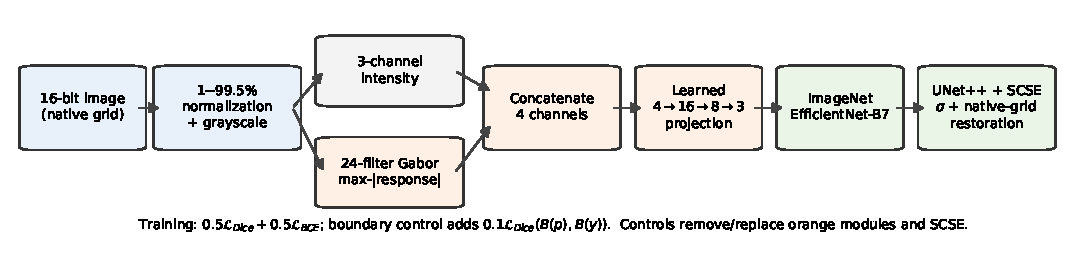
\includegraphics[width=\textwidth]{figures/method_pipeline.pdf}
\caption{Implemented semantic segmentation pipeline. The fixed Gabor bank supplies a maximum-response map, while the learned projection, EfficientNet-B7 encoder, UNet++ decoder, and SCSE blocks are trainable. Matched controls remove or replace the orange components. Predictions are restored to the native grid before evaluation.}
\label{fig:method}
\end{figure*}

\subsection{Losses and sampling}
The common objective is
\begin{equation}
\mathcal L_{seg}=0.5\mathcal L_{Dice}+0.5\mathcal L_{BCE}.
\end{equation}
The explicitly named boundary variant adds $0.1\mathcal L_{Dice}(B(p),B(y))$, where $B(u)=\operatorname{maxpool}_3(u)-\operatorname{minpool}_3(u)$. We make no Tversky or recall-bias claim. Adaptive positive weighting, when audited, uses weight one for zero-positive batches to remain finite.

For the weighted-sampling ablation, let foreground ratio $r_i$, Canny edge ratio $c_i$, and $s_i=1.5$ if $r_i<0.05$ and one otherwise. Sampling with replacement uses $q_i=w_i/\sum_jw_j$ and
\begin{equation}
w_i=\begin{cases}0.3,&r_i\le0.001,\\(2+3r_i)s_i(1+c_i),&r_i>0.001.\end{cases}
\end{equation}
Uniform sampling is used in all main comparisons.

\section{Datasets and experimental design}
\subsection{BBBC039 fluorescence microscopy}
BBBC039v1 contains 200 16-bit $520\!\times\!696$ Hoechst images of U2OS cells, with approximately 23,000 annotated nuclei~\cite{ljosa2012annotated,caicedo2019nucleus}. We use the provider's 100/50/50 train/validation/test partition. No crops or ROIs are generated. Identifiers, decoded-image hashes, and source labels are checked across partitions. Validation contains 49 foreground images and one empty reference; test contains no empty references. Because BBBC039 partially overlaps BBBC038, BBBC038 is not presented as independent validation.

\subsection{TNBC breast histology}
TNBC v1.1 contains 50 H\&E images with nuclear masks from 11 patients~\cite{naylor2019segmentation}. Patient identifiers are extracted from image names and locked before training. Five outer folds are used: test patients $(04,11)$, $(01,02)$, $(09,07)$, $(03,10)$, and $(05,08,06)$, with 11, 10, 9, 9, and 11 images, respectively. For test fold $k$, fold $(k+1)\bmod5$ is validation and the remaining patients are training. Every patient is tested once and no patient appears in more than one partition within a run. Because TNBC labels were viewed during earlier zero-shot analysis, this grouped CV study is exploratory rather than a pristine external confirmation.

\begin{figure*}[t]
\centering
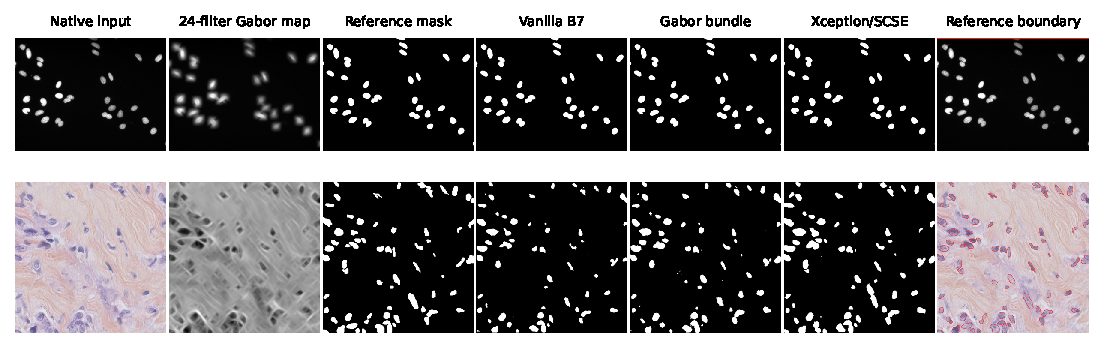
\includegraphics[width=\textwidth]{figures/public_dataset_examples.pdf}
\caption{Real public images and held-out predictions. Top: BBBC039 fluorescence case IXMtest\_I23\_s5\_w1E3053D6B-8CEF-48E3-A6A5-2F0D7C1AA177. Bottom: TNBC case 01\_1. Columns show native input, fixed 24-filter Gabor response, reference mask, vanilla EfficientNet-B7/UNet++ prediction, Gabor/projection/SCSE prediction, Xception/SCSE prediction, and reference boundary overlay. Cases were selected mechanically as the image nearest the three-seed median vanilla Dice; display seed 1 was fixed before visual inspection.}
\label{fig:examples}
\end{figure*}

\subsection{Private UWM lineage}
The private lineage contains 855 valid annotated planes exported from in-house MCF10A confocal $z$-stacks (Zeiss LSM, 40$\times$/1.1 W, 405/461 nm, 0.2506 $\mu$m pixels, 1.0 $\mu$m $z$-step, 16-bit). One trained annotator delineated foreground with expert review; no repeat-annotation agreement study is available. Exact provenance links 334 planes to eight named stacks, while 521 lack retained acquisition identifiers. We therefore retain this data only as a corrected audit, using 23 conservative geometry-defined groups split into 516/133/206 planes (11/5/7 groups), not as independent external validation. No private images are distributed or needed to reproduce the public conclusions.

\subsection{Training protocol}
All public models use seeds 0, 1, and 2; 20 epochs; $512^2$ inputs; batch size 8; AdamW with learning rate $3\times10^{-4}$ and weight decay $10^{-4}$; cosine decay; gradient clipping at one; and identical flips and $90^\circ$ rotations. The best complete native-grid validation Dice chooses the checkpoint. Threshold 0.5, no test-time augmentation, and retention of the final short batch are fixed. BBBC039 has seven component models (21 runs), ten validation-only sensitivity settings (30), and six architecture baselines (18), totaling 69 runs/1,380 epochs. TNBC has three models, five folds, and three seeds, totaling 45 runs/900 epochs. The complete public study therefore contains 114 training runs and 2,280 epochs.

\subsection{Metrics and statistics}
Predictions are restored to native resolution before Dice, IoU, boundary F1 (BF1), surface Dice at two pixels, and bidirectional HD95. A both-empty pair scores Dice, IoU, and BF1 as one and HD95 as zero; a one-empty pair scores overlap and boundary metrics as zero and HD95 as the image diagonal. Foreground and empty strata are reported separately where present.

For BBBC039, each seed is first averaged per image. For TNBC, each patient's images are averaged before the patient-macro endpoint. Ten thousand paired bootstrap resamples form 95\% confidence intervals, two-sided Wilcoxon tests compare paired units, and Holm correction covers the declared comparison family. Seed SD quantifies optimization variation and is not treated as biological sample size.

\section{Results}
\subsection{BBBC039 matched comparison}
Table~\ref{tab:bbbc} reports every matched main or architecture run. The Gabor bundle gains 0.250 Dice points over vanilla B7 (95\% CI 0.197--0.299; Holm-adjusted $p=7.34\times10^{-9}$), with a similar boundary improvement. However, the difference from the strongest matched architecture, UNet++/Xception/SCSE, is $-0.014$ points (95\% CI $-0.047$--0.018; Holm-adjusted $p=.378$). The boundary term and residual fusion do not improve the Gabor bundle. Cellpose-SAM reaches 96.95\% semantic Dice as a frozen contextual reference; unknown pretraining overlap and unequal optimization prevent treating it as a controlled baseline.

\begin{table*}[t]
\centering\small
\caption{BBBC039 official-test performance. Values are three-seed means; Dice reports seed SD. All trained rows use the same split, augmentations, epoch budget, checkpoint rule, threshold, and no TTA.}
\label{tab:bbbc}
\setlength{\tabcolsep}{5.0pt}
\begin{tabular}{@{}lrrrrr@{}}\toprule
Model & Params (M) & Dice (\%) & IoU (\%) & BF1 (\%) & HD95 (px)\\\midrule
Vanilla B7/UNet++ & 68.2 & $96.60\!\pm\!.07$ & 93.44 & 98.53 & 1.32\\
Gabor/projection/SCSE B7 & 68.4 & $96.85\!\pm\!.13$ & 93.91 & 98.63 & 1.28\\
Gabor + boundary & 68.4 & $96.84\!\pm\!.05$ & 93.88 & 98.68 & 1.28\\
SCSE-only B7 & 68.4 & $96.38\!\pm\!.53$ & 93.03 & 98.48 & 1.35\\
Residual Gabor B7 & 68.4 & $96.57\!\pm\!.27$ & 93.39 & 98.52 & 1.31\\
Residual Sobel B7 & 68.4 & $96.44\!\pm\!.48$ & 93.14 & 98.47 & 1.35\\
Residual Gabor + boundary & 68.4 & $96.61\!\pm\!.31$ & 93.46 & 98.58 & 1.29\\\midrule
U-Net/ResNet-34 & 24.4 & $96.73\!\pm\!.29$ & 93.68 & \textbf{98.71} & 1.29\\
U-Net/ResNet-50 & 32.5 & $96.74\!\pm\!.21$ & 93.69 & 98.67 & 1.29\\
UNet++/EfficientNet-B0 & 6.6 & $96.59\!\pm\!.06$ & 93.40 & 98.55 & 1.34\\
UNet++/Xception/SCSE & 35.3 & $\mathbf{96.87\!\pm\!.11}$ & \textbf{93.93} & 98.69 & \textbf{1.27}\\
DeepLabV3+/ResNet-50 & 26.7 & $95.05\!\pm\!.10$ & 90.57 & 96.93 & 1.92\\
FPN/ResNet-50 & 26.1 & $94.97\!\pm\!.28$ & 90.43 & 96.96 & 1.93\\\bottomrule
\end{tabular}
\end{table*}

\subsection{Filter, loss, and sampling sensitivity}
The sensitivity study is locked to validation data and never decodes test images. The eight-orientation/three-frequency reference obtains 96.684\% foreground Dice. Four and 12 orientations yield 96.686\% and 96.664\%; one and five frequencies yield 96.723\% and 96.715\%; $\sigma=3$ and 7 yield 96.541\% and 96.709\%. Sobel, a neutral-edge control, and weighted sampling yield 96.727\%, 96.586\%, and 96.731\%. Weighted sampling improves foreground Dice by only 0.047 points (95\% CI 0.022--0.080) and performs worse on the single empty validation field, so it is not adopted. These small variations do not establish unique optimality of the 24-filter bank.

\subsection{Patient-grouped TNBC training}
Table~\ref{tab:tnbc} gives the new within-dataset study. Vanilla B7 is best at 74.29\% patient-macro Dice, followed by Xception/SCSE at 73.03\%. The Gabor bundle reaches 67.02\% and has much larger seed variation. Its paired difference from vanilla is $-7.26$ Dice points (95\% CI $-9.98$ to $-5.26$; Holm-adjusted $p=.0039$), and its BF1 difference is $-10.40$ points (95\% CI $-13.14$ to $-8.21$; Holm-adjusted $p=.0039$). Against Xception/SCSE, Gabor loses 6.00 Dice points (95\% CI $-7.88$ to $-4.25$; Holm-adjusted $p=.0039$). Thus the fluorescence benefit reverses under breast H\&E acquisition.

\begin{table}[t]
\centering\footnotesize
\caption{TNBC five-fold patient-grouped cross-validation. Endpoints are patient-macro means across 11 held-out patients and three seeds; brackets are 95\% patient-bootstrap CIs.}
\label{tab:tnbc}
\setlength{\tabcolsep}{3.2pt}
\begin{tabular}{@{}lrrr@{}}\toprule
Model & Dice & IoU & BF1\\\midrule
Vanilla B7 & \textbf{.7429} & \textbf{.6001} & \textbf{.6306}\\
95\% CI & [.7148,.7692] & [.5702,.6292] & [.5874,.6731]\\
Gabor B7 & .6702 & .5189 & .5266\\
95\% CI & [.6235,.7104] & [.4751,.5581] & [.4698,.5783]\\
Xception/SCSE & .7303 & .5871 & .5915\\
95\% CI & [.6929,.7641] & [.5480,.6235] & [.5435,.6384]\\\bottomrule
\end{tabular}
\end{table}

\begin{figure*}[t]
\centering
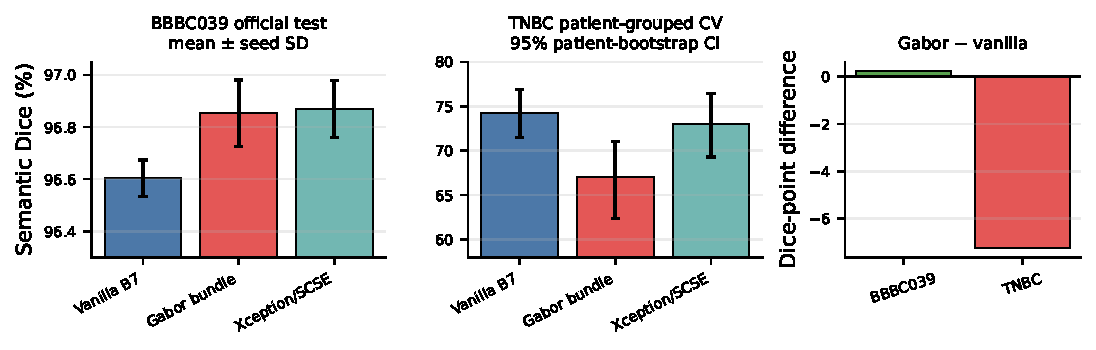
\includegraphics[width=.94\textwidth]{figures/cross_dataset_results.pdf}
\caption{The measured effect changes with acquisition. Left: BBBC039 official split (bars show mean and seed SD). Center: TNBC patient-grouped CV (95\% patient-bootstrap CIs). Right: paired Gabor-minus-vanilla Dice difference. The small positive fluorescence effect becomes a large negative H\&E effect.}
\label{fig:crossdomain}
\end{figure*}

\subsection{Zero-shot polarity stress test}
A BBBC039-trained model is a deliberately difficult transfer test, not a TNBC competitor. Explicit grayscale conversion reproduces the existing input exactly for all 50 TNBC images because the pipeline already converts RGB to grayscale. The vanilla model obtains 8.07\% patient-macro Dice. A single fixed transformation, $x'=255-x$, raises it to 51.30\%, a 43.24-point patient-paired gain (95\% CI 36.55--50.15; Holm-adjusted $p=.00684$), without retraining, threshold fitting, or checkpoint selection. Gabor rises from 2.94\% to 37.66\%. Figure~\ref{fig:polarity} shows the diagnostic. Inversion exposes polarity mismatch but does not solve stain, morphology, or tissue-context shift.

\begin{figure}[t]
\centering
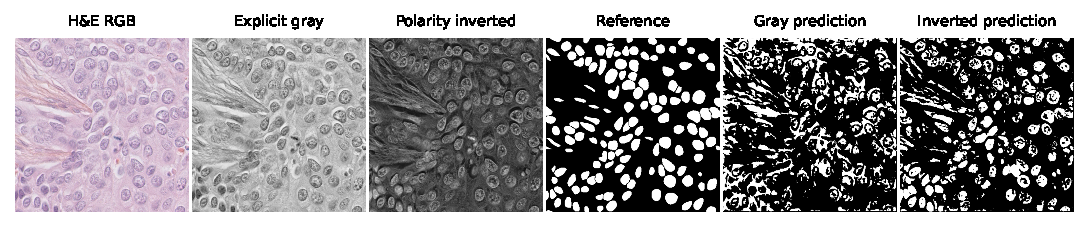
\includegraphics[width=\columnwidth]{figures/tnbc_polarity_example.pdf}
\caption{Fixed zero-shot polarity test on TNBC. The BBBC039-trained model expects bright nuclei; inversion makes dark H\&E nuclei bright and recovers a substantial fraction of overlap. This is a diagnostic, not a trained TNBC result.}
\label{fig:polarity}
\end{figure}

\subsection{Private-result reconciliation}
The rejected manuscript's stored aggregate Dice was 0.9513, but the arithmetic mean of its 128 saved per-image values is 0.9413. Both used a leakage-prone slice split. Under conservative grouped evaluation, the full pipeline obtains 0.9312 Dice (95\% group-bootstrap CI 0.9134--0.9472), vanilla B7 0.9349 (0.9175--0.9515), plain Dice+BCE 0.9366 (0.9199--0.9529), U-Net/ResNet-50 0.9320 (0.9140--0.9502), and frozen Cellpose-SAM 0.9198 (0.9058--0.9321). No full-pipeline superiority remains after group-aware correction. All 855 valid masks contain foreground; the previous statement that 60\% were empty resulted from thresholding binary 0/1 masks at 127.

\subsection{Comparison with published reports}
Tables~\ref{tab:lit_bbbc} and~\ref{tab:lit_tnbc} preserve each paper's reported metric and protocol. They are not rankable leaderboards: some studies use object F1 or AJI, some use cross-validation, some apply instance postprocessing, and none shares our exact patient folds and three-seed schedule. The controlled conclusion comes from Tables~\ref{tab:bbbc} and~\ref{tab:tnbc}; literature values only establish the performance range reported on the same named datasets.

\begin{table*}[t]
\centering\small
\caption{Published BBBC039 context. Ours is trained on the official 100/50/50 split. Differences in task definition and protocol preclude direct significance testing across papers.}
\label{tab:lit_bbbc}
\setlength{\tabcolsep}{5pt}
\begin{tabular}{@{}llll@{}}\toprule
Study & Evaluation description & Reported endpoint & Directly comparable?\\\midrule
Ours, Gabor bundle & Official split; semantic; 3 seeds & Dice .9685; IoU .9391 & Reference\\
Caicedo et al.~\cite{caicedo2019evaluation} & Official split; instance-aware evaluation & Object F1 .898 & No, different metric\\
SegmentGraph~\cite{yi2022segmentgraph} & Official split & Dice .9482; AJI .8680 & Partly\\
ASW framework~\cite{wang2022aswnet} & Expanded-interior evaluation & DICE1 .9645; AJI .9020 & No, altered targets\\
NUSeg~\cite{wickramasinghe2024nuseg} & Five-fold cross-validation & Dice .9693; IoU .9406 & No, different split\\\bottomrule
\end{tabular}
\end{table*}

\begin{table*}[t]
\centering\small
\caption{Published TNBC context. Our result is patient-macro semantic overlap from fixed patient-grouped folds; cited values retain their papers' metrics and protocols.}
\label{tab:lit_tnbc}
\setlength{\tabcolsep}{4.5pt}
\begin{tabular}{@{}llll@{}}\toprule
Study & Method/protocol as reported & Reported endpoint & Directly comparable?\\\midrule
Ours, vanilla B7 & 5 patient folds; 3 seeds & Dice .7429 [.7148,.7692] & Reference\\
DIST~\cite{naylor2019segmentation,kang2020twostage} & Published TNBC evaluation & F1 .824; AJI .585 & No, instance metrics\\
Two-stage stacked U-Net~\cite{kang2020twostage} & Published TNBC evaluation & F1 .806; AJI .621 & No, different split/metric\\
R-SNN~\cite{mahmood2021accurate} & Published TNBC evaluation & Dice .8441; AJI .7332 & No, different protocol\\
FRE-Net~\cite{huang2023frenet} & Published TNBC evaluation & Dice $.8563\!\pm\!.0323$ & No, different protocol\\
MA-Net~\cite{alotaibi2024manet} & Published TNBC evaluation & Dice .7936 & No, different protocol\\
CellTranspose~\cite{he2023celltranspose} & 3--10-shot adaptation & Pixel F1 .670--.757 & No, adapted few-shot setting\\\bottomrule
\end{tabular}
\end{table*}

\section{Discussion}
\subsection{What the evidence supports}
The central result is an interaction, not a universal win. Under fluorescence acquisition, the fixed edge map supplies a small but statistically resolved improvement over one vanilla B7 control. A lower-parameter Xception/SCSE model matches or slightly exceeds it, showing that architecture choice can account for the apparent gain. Under H\&E, the same bundle is significantly worse and less stable. The real-image panels suggest a plausible mechanism: in fluorescence the strongest edges usually outline nuclei, whereas in histology the bank also responds to stain and tissue texture. This visual interpretation is consistent with, but does not itself prove, the measured interaction.

The work is stronger than the rejected version because the principal claim no longer depends on private data or a favorable split. Public data, fixed folds, run manifests, equal budgets, per-image outputs, confidence intervals, statistical tests, boundary metrics, filter sensitivity, and failed configurations are all retained. The method description now matches the implementation: the boundary variant contains an explicit boundary term, and the main loss is Dice+BCE rather than incorrectly interpreted Tversky weighting.

\subsection{What the evidence does not support}
The study does not establish clinical-grade performance, breast-cancer diagnosis, universal cross-modality generalization, or superiority over every published model. Literature tables are contextual because metrics and partitions differ. Semantic masks also cannot justify instance-level claims about touching-nucleus separation. Finally, the 3-D work remains a separate exploratory direction and is not evidence for the 2-D conclusions.

\section{Limitations and next experiments}
TNBC contains only 11 patients, labels had been viewed before the grouped-CV study, and three seeds provide limited optimization sampling. Grayscale intentionally matches the original pipeline but discards diagnostically useful stain information. A confirmatory experiment should preregister preprocessing and compare grayscale, RGB, stain-normalized RGB, and HED channels under identical patient folds, then evaluate once on an unseen external patient cohort. If an instance claim is desired, connected-instance outputs must be evaluated with AJI, panoptic quality, and detection F1 under a defined matching rule. Multi-annotator boundary agreement is also needed to separate model error from reference uncertainty. For the private lineage, original stack identifiers and volume-wise splits must be recovered before any independent-validation claim.

\section{Conclusion}
Across 114 controlled public-data runs and 2,280 training epochs, the Gabor bundle adds 0.25 Dice points on BBBC039 fluorescence but loses 7.26 points on patient-grouped TNBC H\&E. The result converts a narrow benchmark improvement into a more informative finding: explicit edge priors are acquisition-dependent. Equal-budget controls, group-aware splits, and transparent negative results are more consequential to the scientific conclusion than the extra filter channel itself.

\section{Compliance with ethical standards}
BBBC039 is an openly released cell-line benchmark. TNBC is a previously published, de-identified public histology dataset reused without intervention, interaction, access to identifiers, or attempted re-identification. No private patient data are analyzed. The authors must obtain a formal UWM determination and replace this sentence with the exact category, wording, and identifier required by the target venue before submission.

\section{Data and code availability}
The public-data training configurations, fixed patient folds, run manifests, analysis code, per-image metrics, and manuscript sources are available at \url{https://github.com/vkd14/breast-seg-isbi2027}. BBBC039 is available from the Broad Bioimage Benchmark Collection and TNBC v1.1 from its cited public repository. Dataset images are not duplicated in the code release; download scripts and integrity metadata reproduce their placement. Private UWM images are not distributed and are not required for any public-data result.

\section{Acknowledgments and disclosures}
This work was supported by U.S. Department of Energy grant DE-SC0025403. The authors declare no competing interests. OpenAI Codex assisted with repository auditing, analysis scripts, statistical summaries, figure preparation, and language editing. The authors selected the research questions, ran and verified the experiments, inspected all outputs, and take responsibility for the manuscript. Figures contain measured data and real images/predictions, not generated microscopy content.

\bibliographystyle{IEEEbib}
\bibliography{references}
\end{document}
